% !TEX root = ../main.tex

\section{Foundational Monte Carlo Inference Methods}
\label{sec:inf:foundation}

In this section we introduce the key inference methods that form
the basis upon which most Monte Carlo inference schemes are based.  The
key idea at the heart of all Monte Carlo inference methods is to use some form
of proposal distribution that we can easily sample from and then make
appropriate adjustments to achieve (typically approximate) samples from
the posterior.  All methods will require only an unnormalized distribution
\begin{align}
\label{eq:inf:unnorm-target}
\gamma(\theta) = \pi(\theta)Z
\end{align}
as a target where $Z = \int \gamma(\theta) d\theta$.  As such they will apply to
any situation where we desire to sample from an unnormalized 
(or in some cases normalized) distribution, for which
the Bayesian inference setting is a particular case where
$\gamma(\theta) = p(\mathcal{D}|\theta)p(\theta)$ and $Z = p(\mathcal{D})$.
They will, in general, vary only on how samples are proposal
and the subsequent adjustments that are made.  However, this will lead to a
plethora of different approaches, varying substantially in their motivation,
theoretical justification, algorithmic details, and the scenarios for which they
are effective.

\subsection{Rejection Sampling}
\label{sec:inf:foundation:rejection}

Rejection sampling~\citep{robert2004monte} is one of the simplest Monte Carlo 
inference methods and one of the only ones to produce exact samples from 
the target.  Before going into the method itself, we first consider an example to
demonstrate the underlying intuition.  Imagine we want to generate samples 
distributed uniformly over some arbitrary two dimensional shape.  One simple
way of doing this would be to sample uniformly from a box enclosing the
shape and then only taking the samples which fall with the shape.
An example of such sampling by rejection is shown in Figure~\ref{fig:inf:rej-butt}.
As all the samples within the space or distributed uniformly, they are also
uniformly distributed on any subset of the space.  Therefore if we sample
from a space incorporating the area we care about and then only take the samples
that fall within the desired shape, we will generated samples uniformly over
that shape. We can also use this method to estimate the area of the shape by using
the fact that the probability of any one sample falls within the shape is equal to
the ratio of the areas of the shape and the bounding box, namely
\begin{align}
A_{\text{shape}} &= A_{\text{box}}	P(\theta \in \text{shape}) \\
&\approx \frac{A_{\mathrm{box}}}{N} \sum_{n=1}^{N} \ind (\hat{\theta}_n \in \text{shape})
\quad \text{where} \quad \hat{\theta}_n \sim \textsc{Uniform}(\text{box})
\end{align}
where we have used a Monte Carlo estimate for $P(\theta \in \text{shape})$.
Note that the value of $P(\theta \in \text{shape})$ will
dictate the efficiency of our estimation as it represents the \emph{acceptance rate}
of our samples.  In other words, we need to generate on average $1/P(\theta \in \text{shape})$
samples from our proposal for each sample created in the target area.  As we
will show later in Section INSERT, $P(\theta \in \text{shape})$ typically becomes very
small as $\theta$ becomes high dimensional, so this approach will typically only
be effective in low dimensions.

\begin{figure}[t]
	\centering
	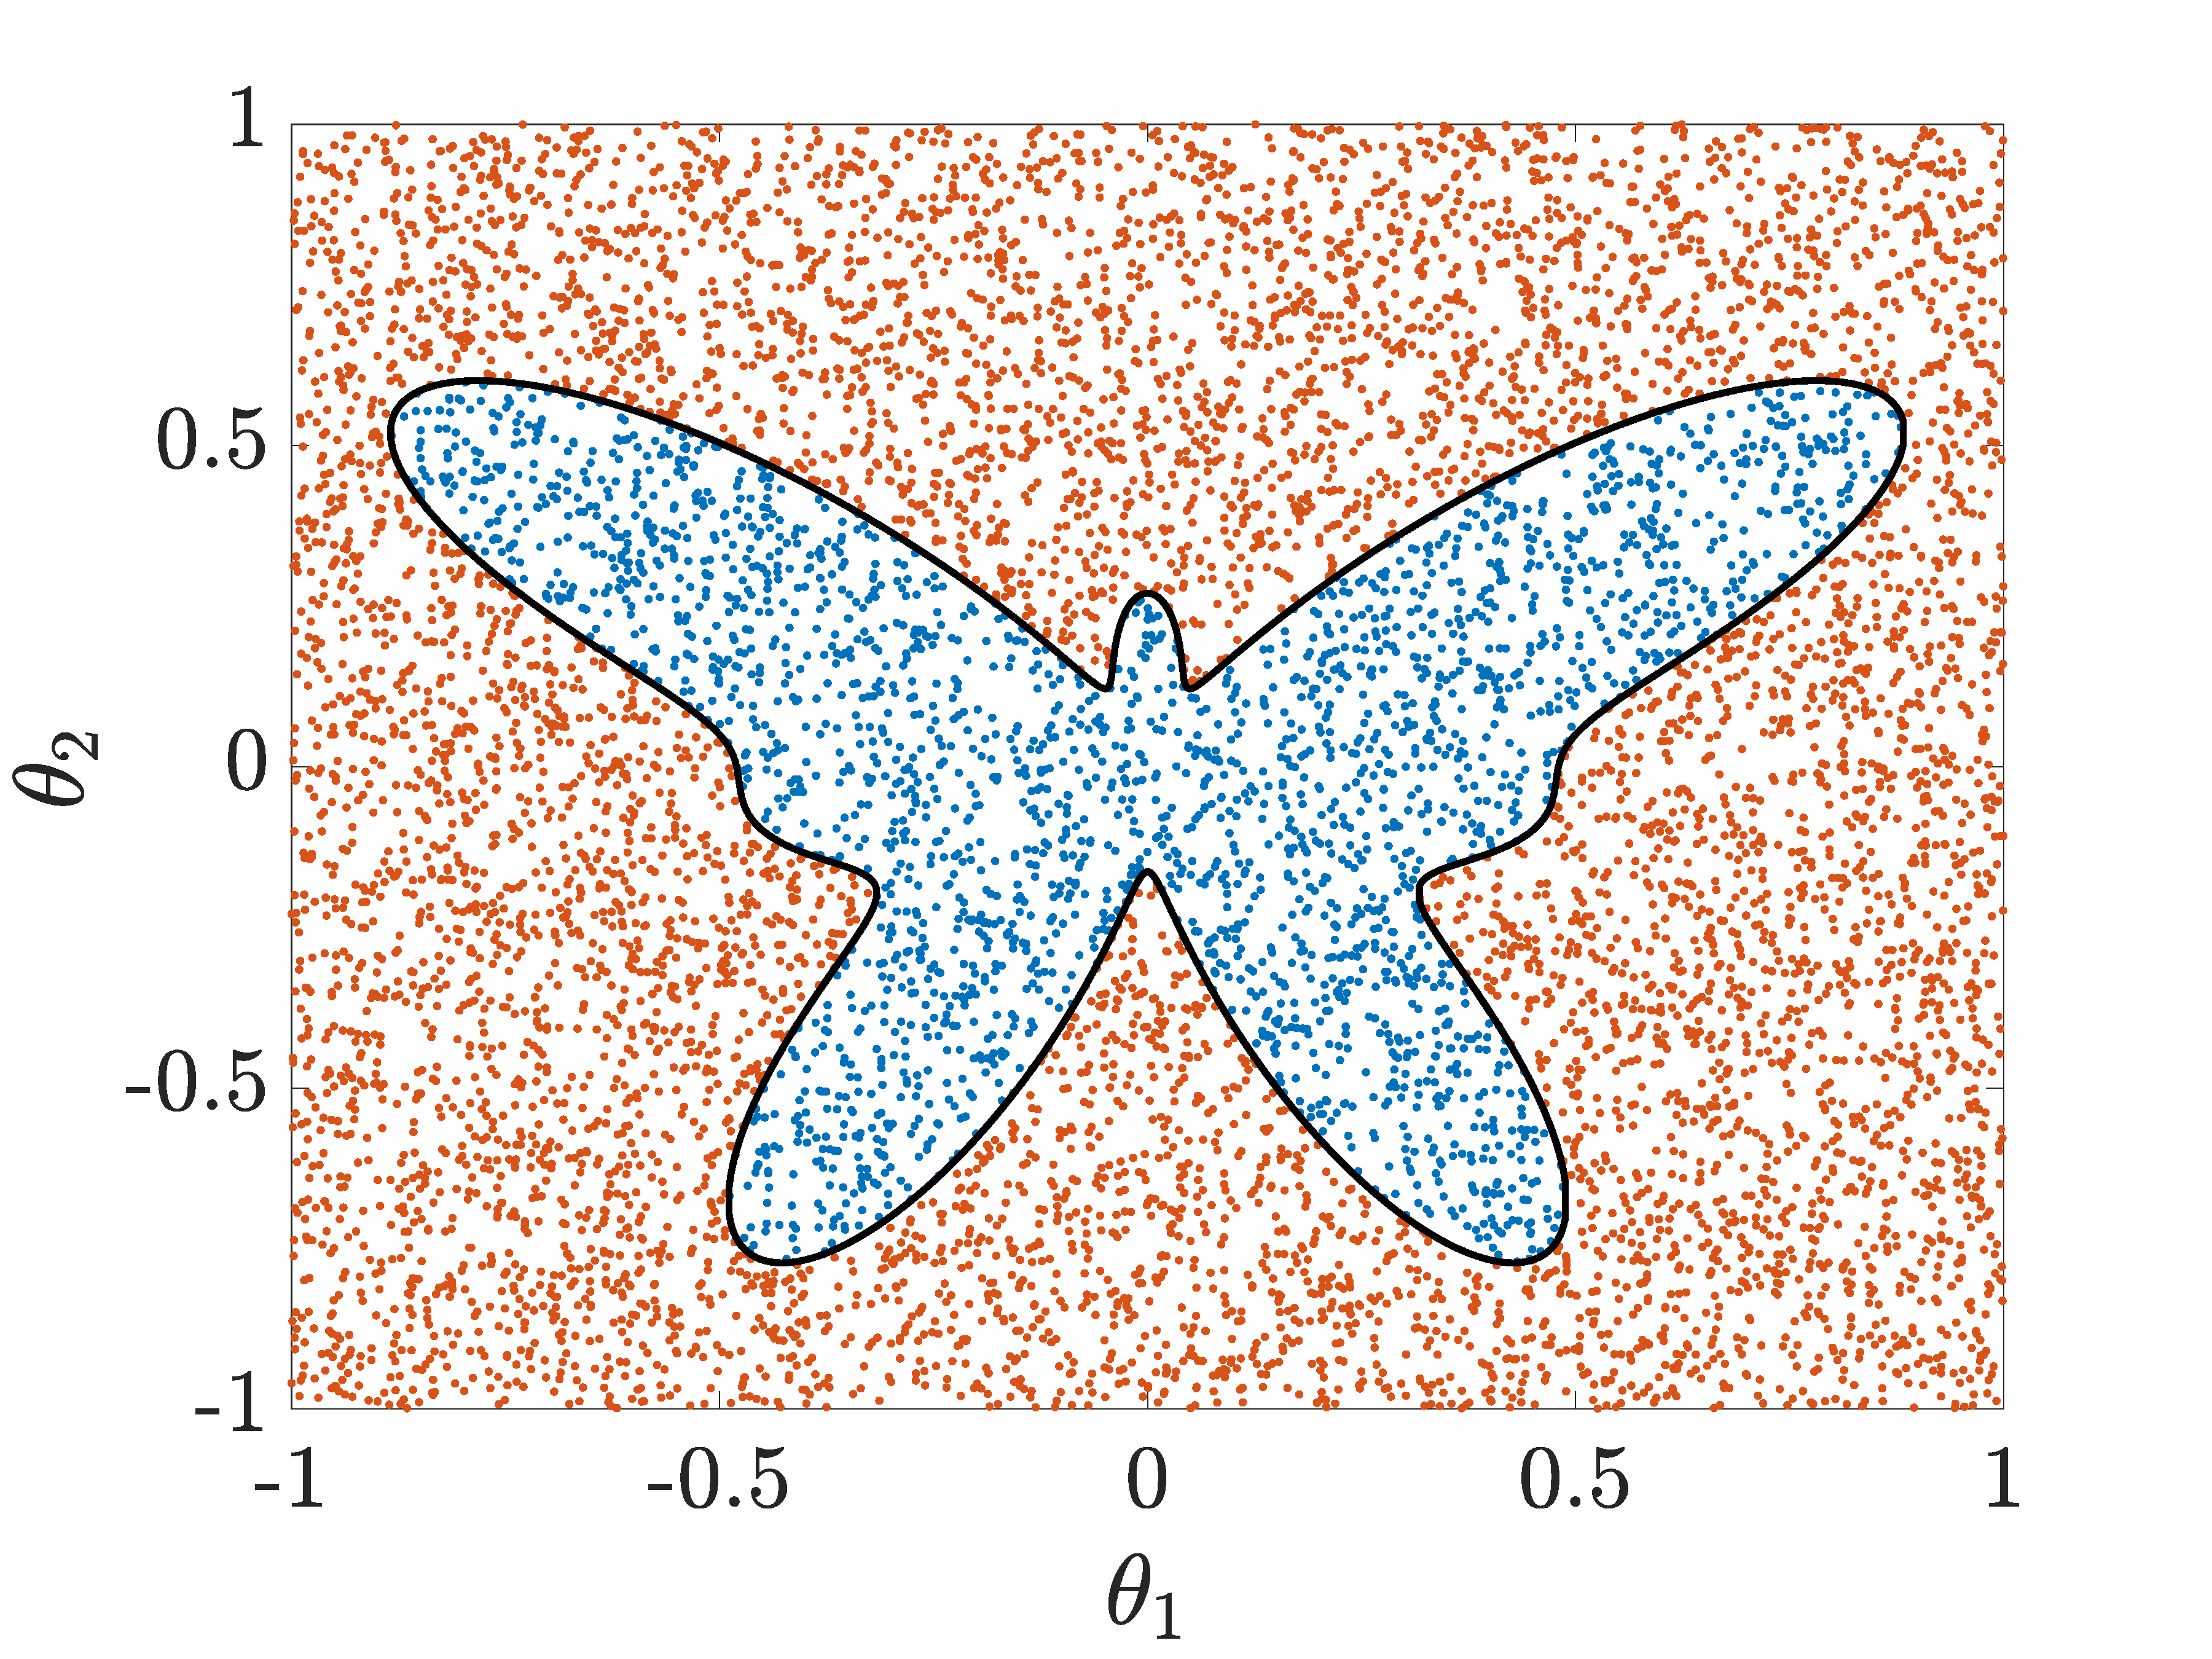
\includegraphics[width=0.6\textwidth]{butterfly}
	\caption{Example of sampling uniformly from an arbitrary shape by 
		rejection.  Here samples are proposed uniformly from the $[-1,1]$
		square.  Any sample falling within the black outline is accepted 
		(blue), otherwise it is rejected (red).  \label{fig:inf:rej-butt}}
\end{figure}

The underlying idea for rejection sampling is that we can sample from any distribution
by sampling uniformly from the hyper-volume under its unnormalized probability density function.
Though this is effectively axiomatic by the definition of a probability density
function with respect to the Lebesgue measure, we can get a non measure-theoretic
intuition for this by considering augmenting a target distribution with a new variable $u$
such that $p(u|\theta) = \textsc{Uniform}(0,\gamma(\theta))$.  Sampling 
$\hat{\theta} \sim \pi(\theta)$ and then $\hat{u}\sim p(u|\theta)$ corresponds to
sampling uniformly from hyper-volume under the probability density function, while we
clearly have that the marginal distribution on $\theta$ is $\pi(\theta)$.

\begin{figure}[t]
	\centering
	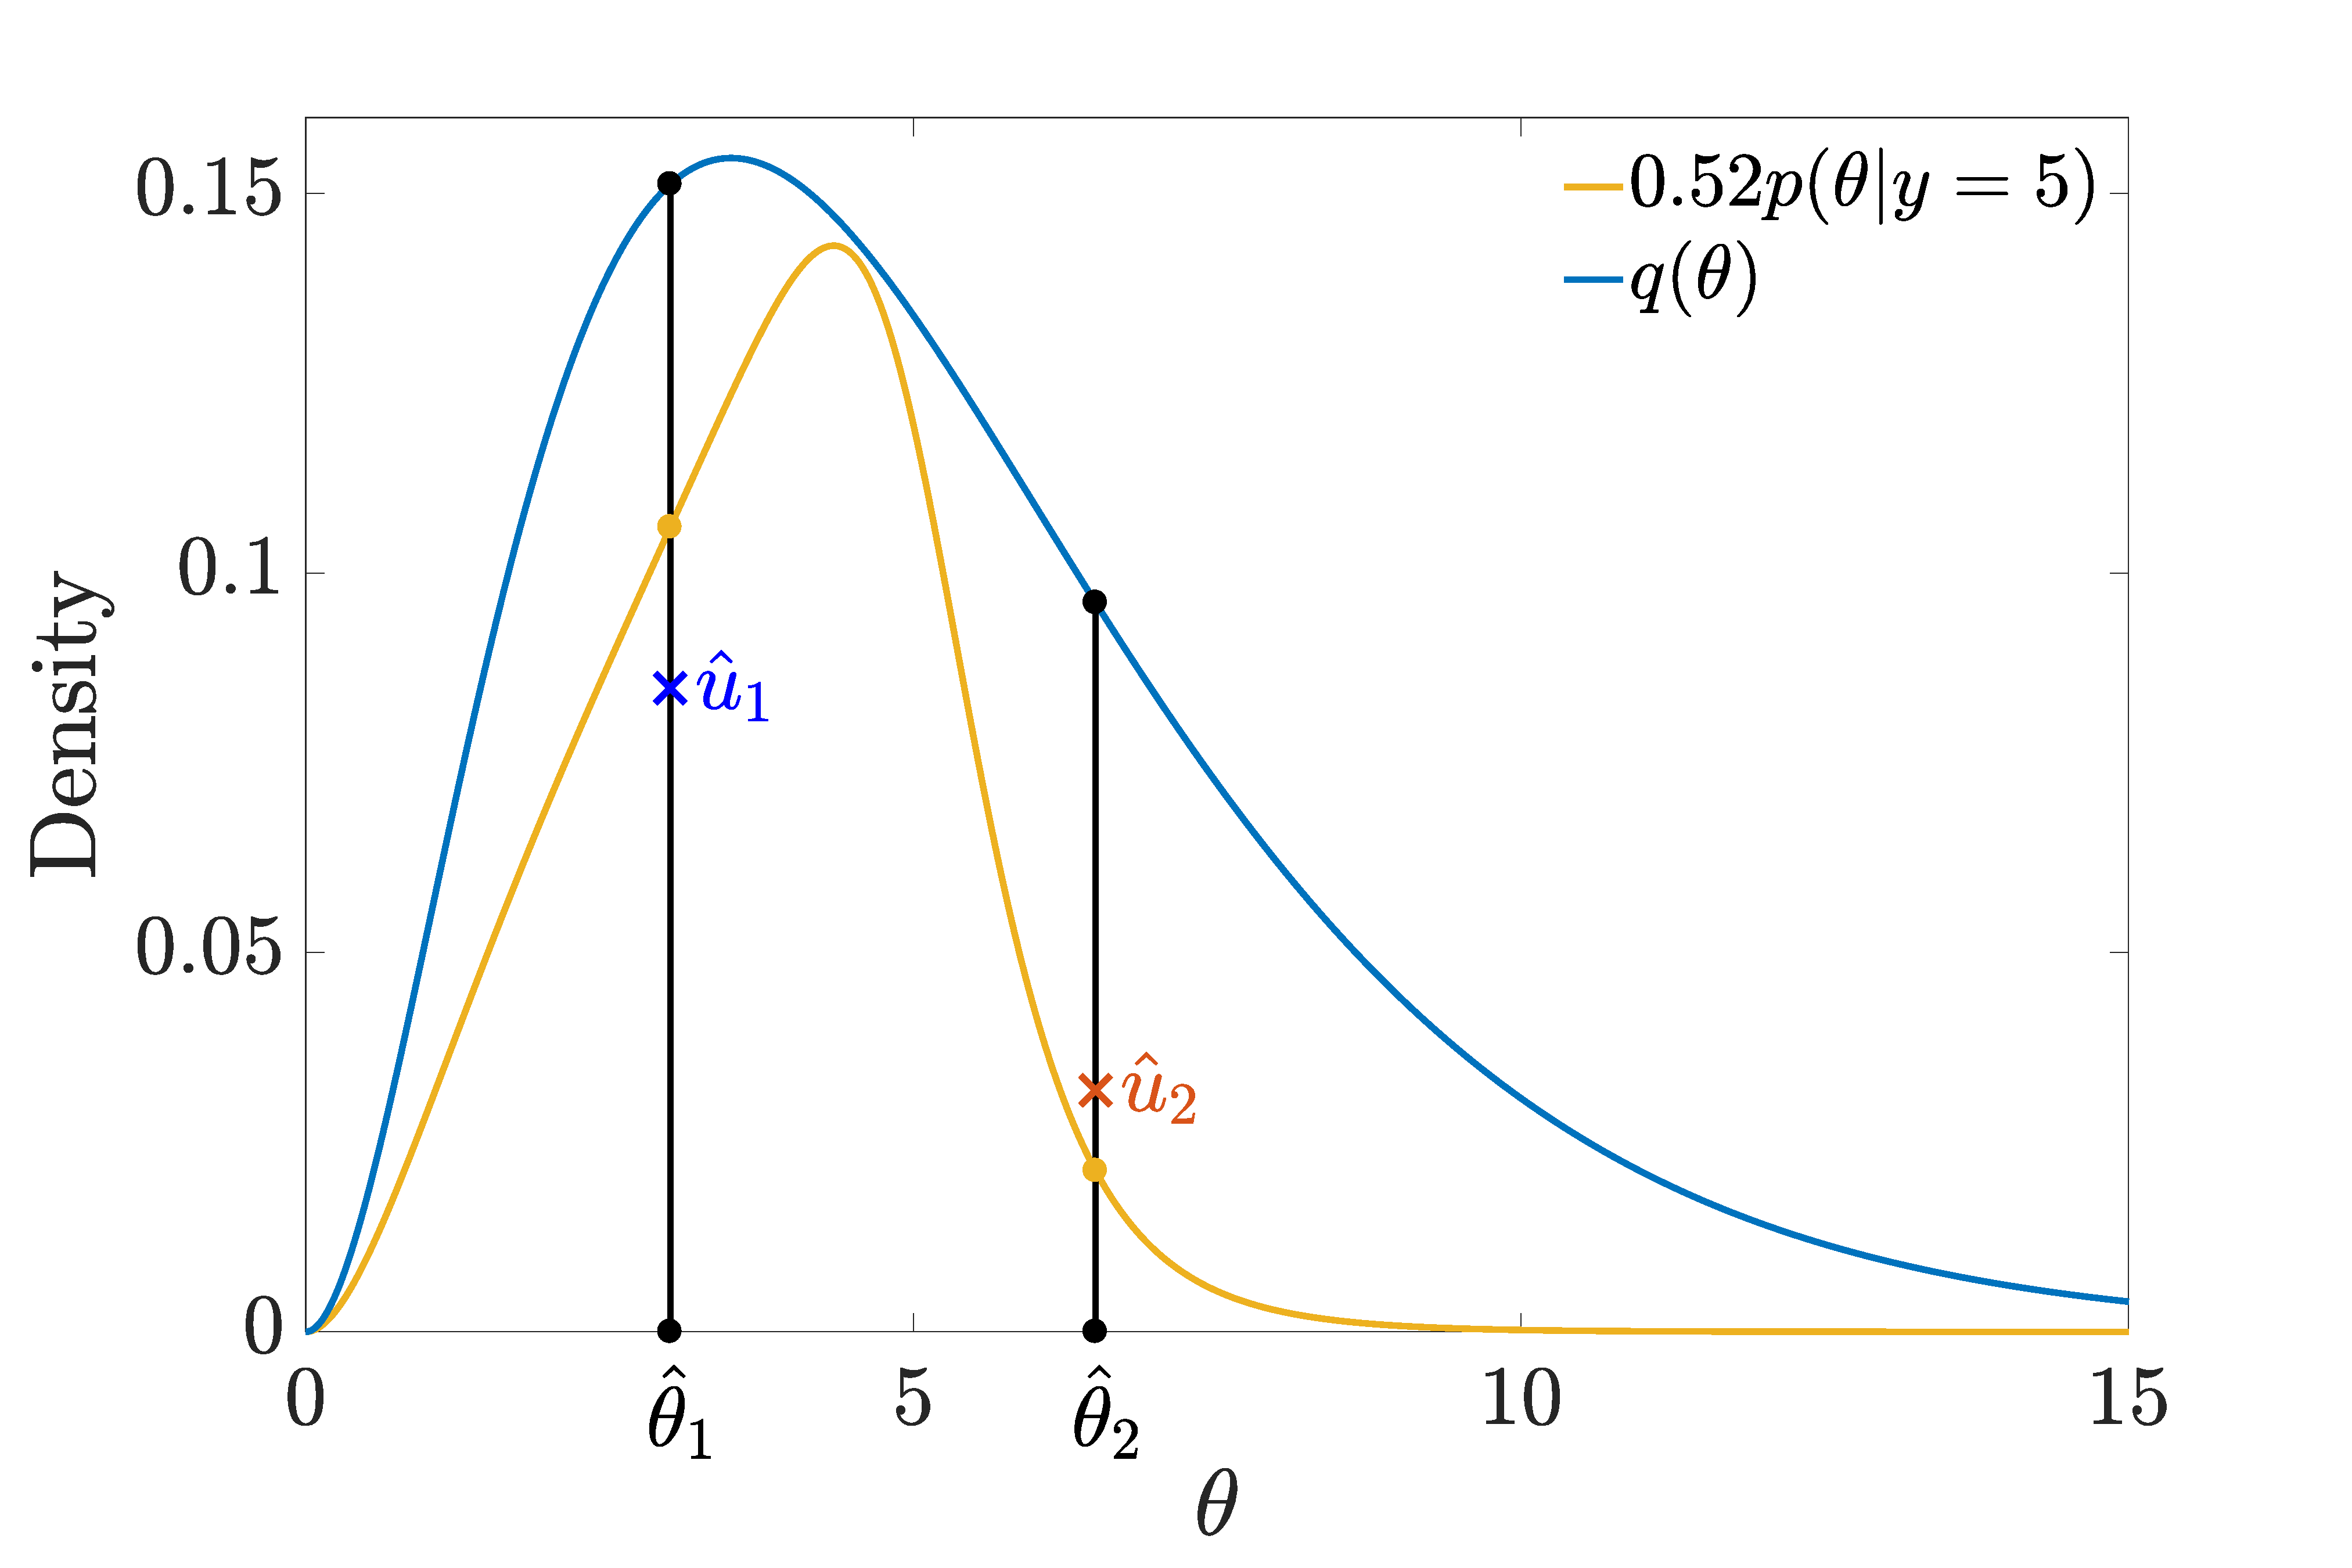
\includegraphics[width=0.7\textwidth]{reject_samp}
	\caption{Demonstration of rejection sampling for problem shown in~\eqref{eq:inf:example}.  
		We first sample $\hat{\theta}\sim q(\theta)$, correspond to the sampling for the distribution
		shown in blue,
		and then sample $\hat{u}\sim \textsc{Uniform}(0,q(\theta))$, corresponding to
		sampling a point uniformly along the black lines for the two shown example values of 
		$\hat{\theta}$.  The point is accepted 
		if $\hat{u} \le C p(\theta | y=5)$ (i.e. if it below the yellow curve) and is 
		otherwise rejected, where we have taken
		$C=0.52$ to ensure $C p(\theta | y=5)\le q(\theta)$ for all theta.
		Here the example sample pair $\{\hat{\theta}_1,\hat{u}_1\}$ is accepted, while
		$\{\hat{\theta}_2,\hat{u}_2\}$ is rejected.  The
		resulting accepted sample pairs will be uniformly sampled from the region under
		the unnormalized target distribution given by the yellow curve and therefore
		the accepted $\hat{\theta}$ will correspond to exact samples from the target.
		 \label{fig:inf:rej-samp}}
\end{figure}

Using this idea, we can sample from any unnormalized distribution by sampling from
an appropriate bounding as per our intuitive example and then accepting only samples
that fall within the hyper-volume of the probability density function. 
More specifically, we define a proposal
distribution $q(\theta)$ which completely envelopes a
scaled version of the unnormalized target distribution $C\gamma(\theta)$ such that 
$q(\theta)\ge C \gamma(\theta)$ for all values of $\theta$ and $C>0$.  We then sample a pair 
$\{\hat{\theta},\hat{u}\}$ by first sampling $\hat{\theta} \sim q(\theta)$ and then
$\hat{u} \sim \textsc{Uniform}(0,q(\theta))$.  The sample is accepted if
\begin{align}
	\label{eq:inf:rej-acc-criteria}
	\hat{u} \le C \gamma(\hat{\theta})
\end{align}
which occurs with an acceptance rate $CZ$ (note that $q(\theta)\ge C \gamma(\theta) \; \forall \theta$
ensures that $C \le 1/Z$).  Note that this can be used to estimate the normalization
constant, corresponding to the marginal likelihood for Bayesian models, by calculating
the empirical estimate of the acceptance rate and dividing this by $C$.
A graphical demonstration of the rejection sampling process is shown in 
Figure~\ref{fig:inf:rej-samp}.

Rejection sampling can be a highly effective sampling or inference method in low dimensions.
In particular, the fact that it generates exact samples from the target distribution can be very
useful.  For example, this characteristic is used to construct efficient samplers for many 
common distributions such as in the ziggurat algorithm~\citep{marsaglia2000ziggurat} often
used for generating Gaussian random variables.  However, its efficiency is critically dependent
on the value of $C$ because it is directly proportional to the acceptance rate.  By proxy, it
is also critically dependent on the proposal $q(\theta)$ as this dictates the minimum possible
value of $C$, namely $C_{\min} = \min_{\theta} q(\theta) Z / \pi(\theta)$.  Note that if 
$q(\theta) = \pi(\theta) \; \forall \theta$ then the acceptance rate will be $1$, while the
more different they are (in terms of $\min_{\theta} q(\theta) / \pi(\theta)$), the lower the
best possible acceptance rate becomes.  In low dimensions, adaptive rejection 
sampling~\citep{gilks1992adaptive} often forms an effective method for adaptively 
learning an effective proposal and corresponding value for $C$, leading to good acceptance
rates.  However, the approach will be very prone to the \emph{curse of dimensionality} as
we discuss in Section~\ref{sec:inf:foundation:curse}, meaning performance cannot be
maintained for higher dimensional problems.

\subsection{Importance Sampling}
\label{sec:inf:foundation:importance}

Importance sampling is another common sampling method that forms the key building block
for many more advance inference schemes.  It is closely related to rejection sampling in that
it samples candidate $\hat{\theta}$ from a proposal $q(\theta)$, but instead of going
through an accept/reject step, it assigns an \emph{importance weight} to each sample.
These importance weights act like correction factors to account for the fact that we sampled
from $q(\theta)$ rather than our target $\pi(\theta)$.

To demonstrate the key idea, consider the problem of calculating an expectation as
per~\eqref{eq:inf:expt}.  If we cannot sample exactly from $\pi(\theta)$ then we cannot
apply~\eqref{eq:inf:mc-est} directly.  However, we can rearrange the form our expectation
to generate a different \mc estimator which we can evaluate directly as follows
\begin{align}
	I:=\E_{\pi(\theta)} \left[f(\theta)\right] &=\int f(\theta) \pi(\theta) d\theta 
	= \int f(\theta) \frac{\pi(\theta)}{q(\theta)} q(\theta) d\theta \nonumber \\
	&\approx \frac{1}{N} \sum_{n=1}^{N} \frac{\pi(\hth_n)}{q(\hth_n)} f(\hat{\theta}_n)
	\quad \text{where} \quad \hat{\theta}_n \sim q(\theta) 	\label{eq:inf:importance}
\end{align}
where $\frac{\pi(\hth_n)}{q(\hth_n)} =: w_n$ is known as an importance weight.
The key trick we have applied is to multiply the integrand by $\frac{q(\theta)}{q(\theta)}$, which
equals $1$
for all points where $q(\theta) \neq 0$.  Thus if $q(\theta) \neq 0$ for all $\theta$ for which
$\pi(\theta) \neq 0$ (to avoid infinite importance weights), this has no effect on the 
expectation.  However, we can informally view the new
formulation as being the expectation of $f(\theta) \frac{\pi(\theta)}{q(\theta)}$ under the
distribution $q(\theta)$.  We can now construct a \mc estimator for this new formulation, 
by choosing $q(\theta)$ to be a distribution we can sample from.

Importance sampling has a number of desirable properties as an inference method.
In particular, it is both unbiased and consistent.  The former can be shown trivially
as follows
\begin{align}
\E \left[\frac{1}{N} \sum_{n=1}^{N} \frac{\pi(\hth_n)}{q(\hth_n)} f(\hat{\theta}_n)\right] &=
\frac{1}{N} \sum_{n=1}^{N} \E _{q(\theta_n)}\left[\frac{\pi(\hth_n)}{q(\hth_n)} f(\hat{\theta}_n)\right] \nonumber \\
&=\E _{q(\theta_1)}\left[\frac{\pi(\hth_1)}{q(\hth_1)} f(\hat{\theta}_n)\right] =
\E _{\pi(\theta)}\left[f(\theta)\right]
\end{align}
where we have effectively stepped backwards through~\eqref{eq:inf:importance}.
Given this unbiasedness result, $L^2$ convergence, and thus convergence in probability,
can be shown in the same manner as~\eqref{eq:inf:LLN-informal} by replacing
each $f(\hth_n)$ with $\frac{\pi(\hth_n)}{q(\hth_n)} f(\hat{\theta}_n)$, leading to the
same result except that $\sigma_{\theta}$ is now
\begin{align}
\label{eq:inf:sigma-imp}
\sigma_{\theta}^2 = \E_{q(\theta)} \left[\left(\frac{\pi(\hth_n)}{q(\hth_n)} f(\hat{\theta}_n)-I\right)^2\right]
= \var_{q(\theta)} \left[\frac{\pi(\theta)}{q(\theta)} f(\theta)\right].
\end{align}
Almost sure convergence of importance sampling can be similarly shown using
the strong law of large numbers.

The form of~\eqref{eq:inf:sigma-imp} provides substantial insight into how
best to set the proposal: we have shown that the mean squared error of an
importance sampler is directly proportional to $\var \left[f(\theta)\pi(\theta)/q(\theta)\right]$,
thus the lower this term is, the better the expected performance of our
estimator.  One obvious question is what is the optimal proposal $q^*(\theta)$?
It turns out that $q^*(\theta) = \frac{\pi(\theta)\left|f(\theta)\right|}
{\int \pi(\theta)\left|f(\theta)\right|d\theta}$
\citep{kahn1953methods,owen2013mc}, which can be
 shown as follows where we will make use of Jensen's inequality
\begin{align}
\var_{q^*(\theta)} &\left[\frac{\pi(\theta)}{q^*(\theta)} f(\theta)\right] =
\E_{q^*(\theta)} \left[\left(\frac{\pi(\theta)}{q^*(\theta)} f(\theta)\right)^2\right]
-\left(\E_{q^*(\theta)} \left[\frac{\pi(\theta)}{q^*(\theta)} f(\theta)\right]\right)^2
\nonumber \\
 &= \int \frac{\pi(\theta)^2 f(\theta)^2}{q^*(\theta)} d\theta
 -I^2 
 = \left(\int \pi(\theta) \left|f(\theta)\right| d\theta\right)^2
 -I^2 \label{eq:inf:opt-q-line2}\\
 &\le \int \left(\frac{\pi(\theta) f(\theta)}{q(\theta)}\right)^2 q(\theta) d\theta
 -I^2 =\var_{q(\theta)} \left[\frac{\pi(\theta)}{q(\theta)} f(\theta)\right] \label{eq:inf:opt-q}.
\end{align}
Here we have shown that the variance for $q^*(\theta)$ is less than or equal to the variance
using an arbitrary $q(\theta)$.  It must therefore be the optimal proposal.
A further point of note is that if $f(\theta)\ge0 \; \forall \theta$, 
then~\eqref{eq:inf:opt-q-line2} will equal zero giving a zero variance estimator:
each importance weight will be equal to the  $I/f(\theta)$ and thus $I$
can be calculated by evaluating a single point.  

Though it will typically be impossible to find $q^*(\theta)$ in practice, it still 
provides a guide as to what constitutes a good proposal -- we want
$\pi(\theta)\left|f(\theta)\right|/q(\theta)$ to be a close to constant as possible.
In particular, we need to be careful to avoid scenarios where 
$\frac{\pi(\theta)\left|f(\theta)\right|}{\int \pi(\theta)\left|f(\theta)\right|d\theta}
\gg q(\theta)$ as this will cause the ratio to explode, leading to high variances.
A consequence of this is that we want $q(\theta)$ to have \emph{light tails}
compared to $\pi(\theta)\left|f(\theta)\right|$ to ensure that the ratio does not
systematically increase as $\theta$ moves away from the modes of $q(\theta)$.
Aside from the clear practical issues, If this requirement does not hold, then
it can easily be the case that $\sigma_{\theta}=\infty$ and thus that the estimator
has infinite variance.  Consider, for example, the case where 
$\pi(\theta) = \mathcal{N}(\theta ; 0,1)$, $f(\theta)=\theta$, and
$q(\theta) = \mathcal{N}(\theta ; 0,s^2)$ (Example 9.1 from~\cite{owen2013mc}).
Noting that the mean, $I$, is zero by symmetry and defining $\nu = \frac{1}{2s^2}-1$, we have that
%, $\mathrm{erf}$ is the error function for which $\mathrm{erf}(\infty)=-\mathrm{erf}(-\infty)=1$)
\begin{align}
\sigma_{\theta}^2 &= \int_{-\infty}^{\infty} \theta^2 \frac{\left(\exp\left(-\theta^2/2\right)/\sqrt{2\pi}\right)^2}
{\exp\left(-\theta^2/\left(2s^2\right)\right)/\sqrt{2\pi s^2}} d\theta
-I^2 \nonumber \\
&= \frac{s}{\sqrt{2\pi}}  \int_{-\infty}^{\infty} \theta^2 \exp \left(\theta^2 \nu\right) d\theta.
%&= \frac{s}{\sqrt{2\pi}}  \int_{-\infty}^{\infty} \theta^2 \exp \left(-\frac{\theta^2}{2}\left(2-\frac{1}{s^2}\right)\right) d\theta
%&= \frac{s}{\sqrt{2\pi}}  \left[
%\frac{\sqrt{\frac{\pi}{2}} \mathrm{erf} \left(\frac{\theta}{\sqrt{2}} \sqrt{2-\frac{1}{s^2}}\right)}
%{\left(2-\frac{1}{s^2}\right)^{3/2}}-\frac{\theta \exp \left(-\frac{\theta^2}{2}\left(2-\frac{1}{s^2}\right)\right) }{\left(2-\frac{1}{s^2}\right)}
%\right]_{\theta=-\infty}^{\theta=\infty} \nonumber \\
%&= \frac{s}{\left(2-\frac{1}{s^2}\right)^{3/2}}
\end{align}
Now this integral is clearly only finite for $\nu < 0$ (as otherwise the integrand
is $+\infty$ and $\theta = \pm \infty$ and finite elsewhere).  Therefore, $\sigma_{\theta}$
is only finite when $s^2>1/2$.  In other words, we only get a finite estimator
in this case if the proposal variance is at least half that of the target distribution $\pi(\theta)$.
The highlights the pitfalls of having insufficiently heavy tails on our proposal.
Overcoming these will typically require careful setup of the proposal on a case-by-case basis,
for example, choosing a distribution type for the proposal that is known to have heavier tails 
than $\pi(\theta)$.

\todo[inline]{Example figure?}

\subsubsection{Self-Normalized Importance Sampling}
\label{sec:inf:foundation:importance:self-norm}

In the previous section we presumed that we have access to a normalize version of the target
$\pi(\theta)$.  Typically this will not be the case and we will only have access to an
unnormalized target $\gamma(\theta)=\pi(\theta)Z$ as per~\eqref{eq:inf:unnorm-target},
for example only having access to the joint rather than the posterior in the Bayesian inference setting.
In a less common but still plausible situation, it may also only be possible to evaluate the proposal
up to a normalization constant.
We now show how one can still use importance sampling in these scenarios, by
\emph{self-normalizing} the importance weights.

The idea point for self-normalized importance sampling (SNIS) is that the weights also provide
an unbiased estimate of the marginal likelihood
\begin{align}
Z_N &= \frac{1}{N} \sum_{n=1}^{N} w_n, \\
\E [Z_N] &= \frac{1}{N} \sum_{n=1}^{N} \E[w_n] =\E_{q(\hth_1)}[\gamma(\hth_1)/q(\hth_1)] = Z,
\end{align}
that can thus 

Strangely, even when the normalization constant
is known, the self-normalized importance sampler can still be lower variance~\cite{owen2013mc}.



\todo[inline]{Unweighted samples through resampling}


\subsubsection{Unknown $f$}
\label{sec:inf:foundation:importance:unk-f}

So far we have assumed that we are using importance sampling to calculate an expectation 
of a known function.  In practice, there will be many scenarios, particularly in the Bayesian inference setting,
where $f(\theta)$ is not known ahead of time and we instead desire to generate samples
for some future unknown use.  For example, in Section INSERT we will introduce the concept
of \emph{sequential Monte Carlo} where we will typically have multiple importance sampling steps
before any target function is itself evaluated.
When no $f(\theta)$ is specified we can carry out importance sampling in the
same fashion, sampling from $q (\theta)$ and returning a set of \emph{weighted} samples
$\{\hth_n,w_n\}_{n=1:N}$ where the weights are equal to $\gamma(\hth_n) / q(\hth_n)$ as before.
Here we can think of importance sampling as approximating the posterior with a series of deltas
functions, namely
\begin{align}
\label{eq:in:imp-post-est}
\pi (\theta) \approx \hat{\pi}(\theta) := \sum_{n=1}^{N} \bar{w}_n \delta_{\hth_n} (\theta)
\end{align}
where $\bar{w}_n$ are the normalized importance weights such that $\sum_{n=1}^N\bar{w}_n = 1$
and $\delta_{\hth_n} (\theta)$ are delta functions centred at $\hth_n$.

As we will show in Section INSERT, importance weights are multiplicative when doing conditional
sampling: if we sample $\hth_n \sim q_1(\theta)$ then $\hat{\phi}_n | \hth_n \sim q_2(\phi | \hth_n)$
when targeting $\gamma_1(\theta)\gamma_2(\phi|\theta)$ then the importance weight is 
\begin{align}
\label{eq:inf:prod-imp-weights}
\frac{\gamma_1(\hth_n)\gamma_2(\hat{\phi}_n|\hth_n)}{q_1(\hth_n)q_2(\hat{\phi}_n | \hth_n)}
=\frac{\gamma_1(\hth_n)}{q_1(\hth_n)}
\times\frac{\gamma_2(\hat{\phi}_n|\hth_n)} {q_2(\hat{\phi}_n | \hth_n)}= w_{n,1} \times w_{n,2}.
\end{align}
This is known as sequential importance sampling and means that we can propagate importance
weighted samples through a computational system and retain a valid importance
sampler with the standard properties such as unbiasedness and consistency.\footnote{Note that
	this does not apply to the \emph{nested estimation} case as we discuss in
	Chapter~\ref{chp:nest}.} 

Again a natural question in this ``unknown $f$'' setting is what is the optimal proposal $q^*(\theta)$?
This is a somewhat more challenging and subjective question that when $f$ is known as the
optimality will depend on what the samples are eventually used for.  In particular, even if we do
not known $f$ precisely, it may be the case that we believe some $f$ are more likely than others or we
may know that $f$ lives within some space of possible functions, for example functions that have
a countable number of discontinuities.  One simple, but insightful approach, is to consider the 
\emph{minimax} optimal proposal, i.e. the proposal that has the minimum variance it $f$ is the
most adversarial possible function for that proposal.  Imagine that we have $N$ independently drawn weighted samples
$\{\hth_n,w_n\}_{n=1:N}$, which thus have $N$ corresponding evaluations $f_n := f(\hth_n)$.
The variance of our estimator is now

OHagan


\subsection{The Curse of Dimensionality}
\label{sec:inf:foundation:curse}

\todo[inline]{Go back to the square-circle case to explain the curse of dimensionality.  Whole
	section on curse of dimensionality?}

\subsection{Markov Chain Monte Carlo}
\label{sec:inf:foundation:mcmc}

\subsection{Gibbs Sampling}
\label{sec:inf:foundation:gibbs}